\documentclass[12pt]{article}
\usepackage{graphicx}
\usepackage{amsmath}
\usepackage{mathtools}
\usepackage{gensymb}
\usepackage{tabularx}
\usepackage{array}
\usepackage[latin1]{inputenc}
\usepackage{fullpage}
\usepackage{color}
\usepackage{array}
\usepackage{longtable}
\usepackage{calc}
\usepackage{multirow}
\usepackage{hhline}
\usepackage{ifthen}
\usepackage{lscape}
\usepackage{float}
\usepackage{amssymb}

\newcommand{\mydet}[1]{\ensuremath{\begin{vmatrix}#1\end{vmatrix}}}
\providecommand{\brak}[1]{\ensuremath{\left(#1\right)}}
\providecommand{\norm}[1]{\left\lVert#1\right\rVert}
\providecommand{\abs}[1]{\left\vert#1\right\vert}
\newcommand{\solution}{\noindent \textbf{Solution: }}
\newcommand{\myvec}[1]{\ensuremath{\begin{pmatrix}#1\end{pmatrix}}}
\let\vec\mathbf

\def\inputGnumericTable{}

\begin{document}
\begin{center}
\textbf\large{OPTIMIZATION}

\end{center}
\section*{Excercise 10.3}

Q.3.2 Reduce the equation $y-2=0$ into normal form. Find the perpendicular distances from the origin and angle between perpendicular and the positive x-axis.

\solution
The given equation can be written as
\begin{align}
	\label{eq:eq1}
	\myvec{0&1}\vec{x} &= 2\\
	\vec{n} &= \myvec{0\\1}\\
	\vec{m} &= \myvec{1\\0}
\end{align}
Equation \eqref{eq:eq1} can be represented in parametric form as
\begin{align}
	\label{eq:eq2}
	\vec{x} = \vec{A}+\lambda\vec{m}
\end{align}
Here, $\vec{A}$ is a point on the given line. We choose
\begin{align}
	\vec{A} &= \myvec{2\\2}\\
	\label{eq:line}
	\eqref{eq:eq2} \implies \vec{x} &= \myvec{2\\2}+\lambda\myvec{1\\0}
\end{align}
Let $\vec{O}$ be the origin. The perpendicular distance will be the minimum distance from $\vec{O}$ to the line. Let $\vec{P}$ be the foot of perpendicular. This problem can be formulated as an optimization problem as follows:
\begin{align}
	& \min_{\vec{x}}\norm{\vec{x}-\vec{O}}^2\\
	& \implies \min_{\lambda}\norm{\myvec{2\\2}+\lambda\myvec{1\\0}-\myvec{0\\0}}^2\\
	& \implies \min_{\lambda}\norm{\myvec{\lambda+2\\2}}^2\\
	\implies f\brak{\lambda} &= \brak{\lambda+2}^2+4\\
	\label{eq:eq3}
	&= \lambda^2+4\lambda+8
\end{align}
$\because$ the coefficient of $\lambda^2>0$, equation \eqref{eq:eq3} is a convex function
\begin{align}
	\label{eq:eq4}
	f^\prime\brak{\lambda} = 2\lambda+4
\end{align}
\begin{enumerate}
\item Computing $\lambda_{min}$ using Derative method:
\begin{align}
	f^{\prime\prime}\brak{\lambda} &= 2\\
	\because f^{\prime\prime}\brak{\lambda}>0,f\prime\brak{\lambda_{min}}=0, for \lambda_{min}\\
	f^{\prime} = 2\lambda+4&=0\\
	\therefore \lambda_{min} &= -2
\end{align}
\item Computing $\lambda_{min}$ using Gradient Descent method:
\begin{align}
	\lambda_{n+1} = \lambda_n - \alpha\nabla f\brak{\lambda_n}
\end{align}
Choosing
\begin{enumerate}
\item $\alpha$ = 0.001
\item precision = 0.0000001
\item n = 10000000
\item $\lambda_0$ = 4
\begin{align}
	\lambda_{min} = -2
\end{align}
\end{enumerate}
\end{enumerate}
Both methods yield same value of $\lambda_{min}$. Substituting this value in equation \eqref{eq:line}
\begin{align}
	\vec{x}_{min} &= \vec{P} = \myvec{2\\2}+\brak{-2}\myvec{1\\0}\\
	&= \myvec{0\\2}\\
	OP &= \norm{\vec{P}-\vec{O}}\\
	&= \norm{\myvec{0\\2}-\myvec{0\\0}}\\
	&= 2
\end{align}
The angle $\theta$ made by this perpendicular with x-axis is given by
\begin{align}
	\theta &= \tan^{-1}{\brak{\frac{2}{0}}}\\
	&= 90\degree
\end{align}
The normal form of equation for straight line is given by 
\begin{align}
	\myvec{\cos{90}\degree&\sin{90}\degree}\vec{x} = 0
\end{align}
See figure \ref{fig:Fig1} and figure \ref{fig:Fig2}
\begin{figure}[!h]
	\begin{center} 
	    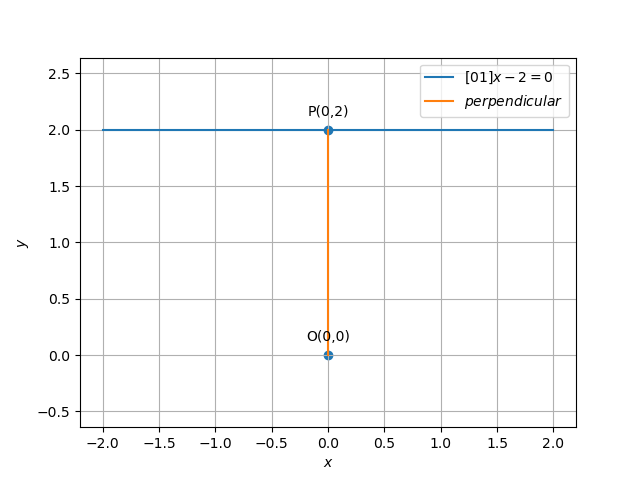
\includegraphics[width=\columnwidth]{figs/opt1}
	\end{center}
\caption{}
\label{fig:Fig1}
\end{figure}
\begin{figure}[!h]
	\begin{center} 
	    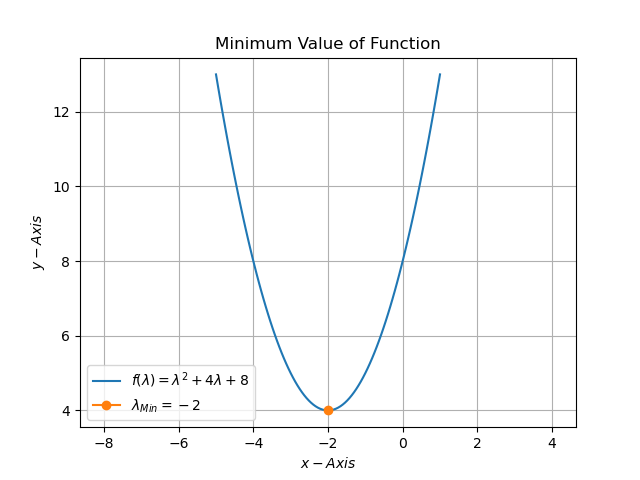
\includegraphics[width=\columnwidth]{figs/opt2}
	\end{center}
\caption{}
\label{fig:Fig2}
\end{figure}

\end{document}







